% ==========================================================================
% HELIX Platform – Use Case Descriptions
% Aligned with SRS and Use Case Diagram (PoC)
% ==========================================================================
\documentclass[12pt,a4paper]{report}

\usepackage[T1]{fontenc}
\usepackage[utf8]{inputenc}
\usepackage[english]{babel}
\usepackage{geometry}
\usepackage{setspace}
\usepackage{microtype}
\usepackage{parskip}
\usepackage{xcolor}
\usepackage{booktabs}
\usepackage{array}
\usepackage{float}
\usepackage{fancyhdr}
\usepackage{titlesec}
\usepackage{enumitem}
\usepackage{tcolorbox}
\usepackage{hyperref}
\usepackage{longtable}
\usepackage{graphicx}

\geometry{a4paper, top=2cm, bottom=2cm, left=2cm, right=2cm, headheight=15pt}

% ── Colors ───────────────────────────────────────────────────────────────
\definecolor{helixpurple}{HTML}{3C3489}
\definecolor{helixpurplelight}{HTML}{EEEDFE}
\definecolor{helixpurplemid}{HTML}{5A50B0}
\definecolor{helixteal}{HTML}{0F6E56}
\definecolor{helixteallight}{HTML}{E1F5EE}
\definecolor{helixamber}{HTML}{7A4A00}
\definecolor{helixamberlight}{HTML}{FDF3DC}
\definecolor{helixgray}{HTML}{3A3A38}
\definecolor{helixgraylight}{HTML}{F4F3EF}
\definecolor{helixborder}{HTML}{CCCAC0}
\definecolor{textsecondary}{HTML}{5A5958}

% ── tcolorbox ────────────────────────────────────────────────────────────
\tcbuselibrary{skins,breakable}

\newtcolorbox{ucbox}[2][]{
    enhanced, breakable,
    colback=helixpurplelight, colframe=helixpurple,
    fonttitle=\bfseries\small\color{white},
    coltitle=white,
    attach boxed title to top left={yshift=-2mm, xshift=6pt},
    boxed title style={colback=helixpurple, colframe=helixpurple, arc=3pt},
    title=#2,
    left=8pt, right=8pt, top=10pt, bottom=8pt,
    arc=5pt, boxrule=0.6pt, #1
}

\newtcolorbox{successbox}[1][]{
    enhanced, breakable,
    colback=helixteallight, colframe=helixteal,
    fonttitle=\bfseries\small\color{helixteal},
    left=8pt, right=8pt, top=6pt, bottom=6pt,
    arc=4pt, boxrule=0.6pt, #1
}

\newcommand{\ucfield}[2]{%
    \noindent\textbf{\color{helixpurplemid}#1:}\quad #2\par\medskip
}

% ── Section styling ──────────────────────────────────────────────────────
\titleformat{\chapter}[block]
{\normalfont\LARGE\bfseries\color{helixpurple}}
{\thechapter.}{12pt}{}
[\vspace{3pt}\color{helixborder}\rule{\linewidth}{0.6pt}\vspace{6pt}]

\titleformat{\section}
{\normalfont\large\bfseries\color{helixgray}}
{\thesection}{10pt}{}

\titlespacing*{\chapter}{0pt}{10pt}{22pt}
\titlespacing*{\section}{0pt}{16pt}{6pt}

% ── Header / Footer ──────────────────────────────────────────────────────
\pagestyle{fancy}
\fancyhf{}
\renewcommand{\headrulewidth}{0.4pt}
\renewcommand{\footrulewidth}{0.4pt}
\fancyhead[L]{\small\color{textsecondary}\scshape{HELIX Platform}}
\fancyhead[R]{\small\color{textsecondary}Use Case Descriptions}
\fancyfoot[C]{\small\color{textsecondary}\thepage}
\fancyfoot[R]{\small\color{textsecondary}2025--2026}

\newcolumntype{L}[1]{>{\raggedright\arraybackslash}p{#1}}
\newcolumntype{C}[1]{>{\centering\arraybackslash}p{#1}}

\setlist[itemize]{leftmargin=1.5em, itemsep=2pt, topsep=3pt}
\setlist[enumerate]{leftmargin=1.7em, itemsep=2pt, topsep=3pt}

\hypersetup{
    colorlinks=true, linkcolor=helixpurple,
    urlcolor=helixteal, citecolor=helixgray,
    pdftitle={HELIX -- Use Case Descriptions},
    pdfauthor={Yasseene}
}

% ==========================================================================
\begin{document}
\setstretch{1.2}

% ── Cover ──────────────────────────────────────────────────────────────────
\begin{titlepage}
    \thispagestyle{empty}
    \noindent\colorbox{helixpurple}{%
        \parbox{\dimexpr\textwidth+2\fboxsep\relax}{%
            \vspace{8pt}
            \hspace{8pt}\textcolor{white}{\small\scshape{Use Case Descriptions --- PoC Version}}
            \vspace{8pt}
        }%
    }
    \vspace{3cm}
    \begin{center}
        {\fontsize{52}{60}\selectfont\bfseries\color{helixpurple} HELIX}\\[10pt]
        {\Large\color{textsecondary}Use Case Textual Descriptions}\\[8pt]
        \color{helixborder}\rule{0.65\textwidth}{0.5pt}\\[30pt]
    \end{center}
    \begin{center}
        \begin{tabular}{L{5.2cm} L{7.5cm}}
            \toprule
            \textbf{Document Type}    & Use Case Descriptions \\
            \midrule
            \textbf{Project Phase}    & Proof of Concept (PoC) \\
            \textbf{Document Version} & 1.0 \\
            \textbf{Academic Year}    & 2025 -- 2026 \\
            \textbf{Author}           & Yasseene \\
            \textbf{Classification}   & Academic --- Confidential \\
            \bottomrule
        \end{tabular}
    \end{center}
    \vfill
    \noindent\colorbox{helixgraylight}{%
        \parbox{\dimexpr\textwidth+2\fboxsep\relax}{%
            \vspace{8pt}
            \hspace{8pt}\small\color{textsecondary}
            Tek-Up University \hfill Ariana, Tunisia \hfill Academic Year 2025--2026
            \vspace{8pt}
        }%
    }
\end{titlepage}

{
    \hypersetup{linkcolor=black}
    \tableofcontents
    \thispagestyle{empty}
}
\clearpage

% ══════════════════════════════════════════════════════════════════════════
% INTRODUCTION
% ══════════════════════════════════════════════════════════════════════════
\chapter*{Introduction}
\addcontentsline{toc}{chapter}{Introduction}

This document provides textual descriptions for all use cases modelled in the
\textbf{HELIX Platform Use Case Diagram}. Each description follows the standard academic
template: \textit{Name, Actors, Preconditions, Postconditions, Main Scenario,} and
\textit{Alternative Scenarios}. Sub-flow use cases (\texttt{<<include>>} / \texttt{<<extend>>})
are grouped with their parent for conciseness.

\section*{Actors}

\begin{center}
    \begin{tabular}{C{1.0cm} L{3.2cm} L{6.5cm}}
        \toprule
        \textbf{ID} & \textbf{Actor} & \textbf{Description} \\
        \midrule
        A0 & Authenticated User & Abstract generalisation; shared capabilities inherited by all authenticated roles \\
        A1 & Administrator & Platform and user management authority \\
        A2 & Blue Team Operator & SOC analyst; monitors events, manages incidents \\
        A3 & Red Team Operator & Penetration tester; executes offensive tools \\
        A4 & Purple Team Operator & Senior hybrid engineer; inherits Blue + Red capabilities \\
        A5 & Visitor & Unauthenticated user; browses public content, registers, logs in \\
        A6 & Learner & Authenticated student; studies, tracks progress, takes notes \\
        A7 & Detection Engine & Autonomous system actor; runs the detection pipeline \\
        \bottomrule
    \end{tabular}
\end{center}

\section*{Use Case Groups}

\begin{enumerate}
    \item Access Control (UC-01 to UC-06)
    \item Security Operations (UC-07 to UC-10)
    \item Detection Pipeline (UC-11 to UC-16)
    \item Red Team Orchestration (UC-17 to UC-20)
    \item Collaboration \& Knowledge Base (UC-21 to UC-26)
    \item Learner Workspace (UC-27 to UC-30)
    \item AI Assistance (UC-31 to UC-33)
\end{enumerate}

% ══════════════════════════════════════════════════════════════════════════
% USE CASE DIAGRAM
% ══════════════════════════════════════════════════════════════════════════
\clearpage
\begin{figure}[H]
    \centering
    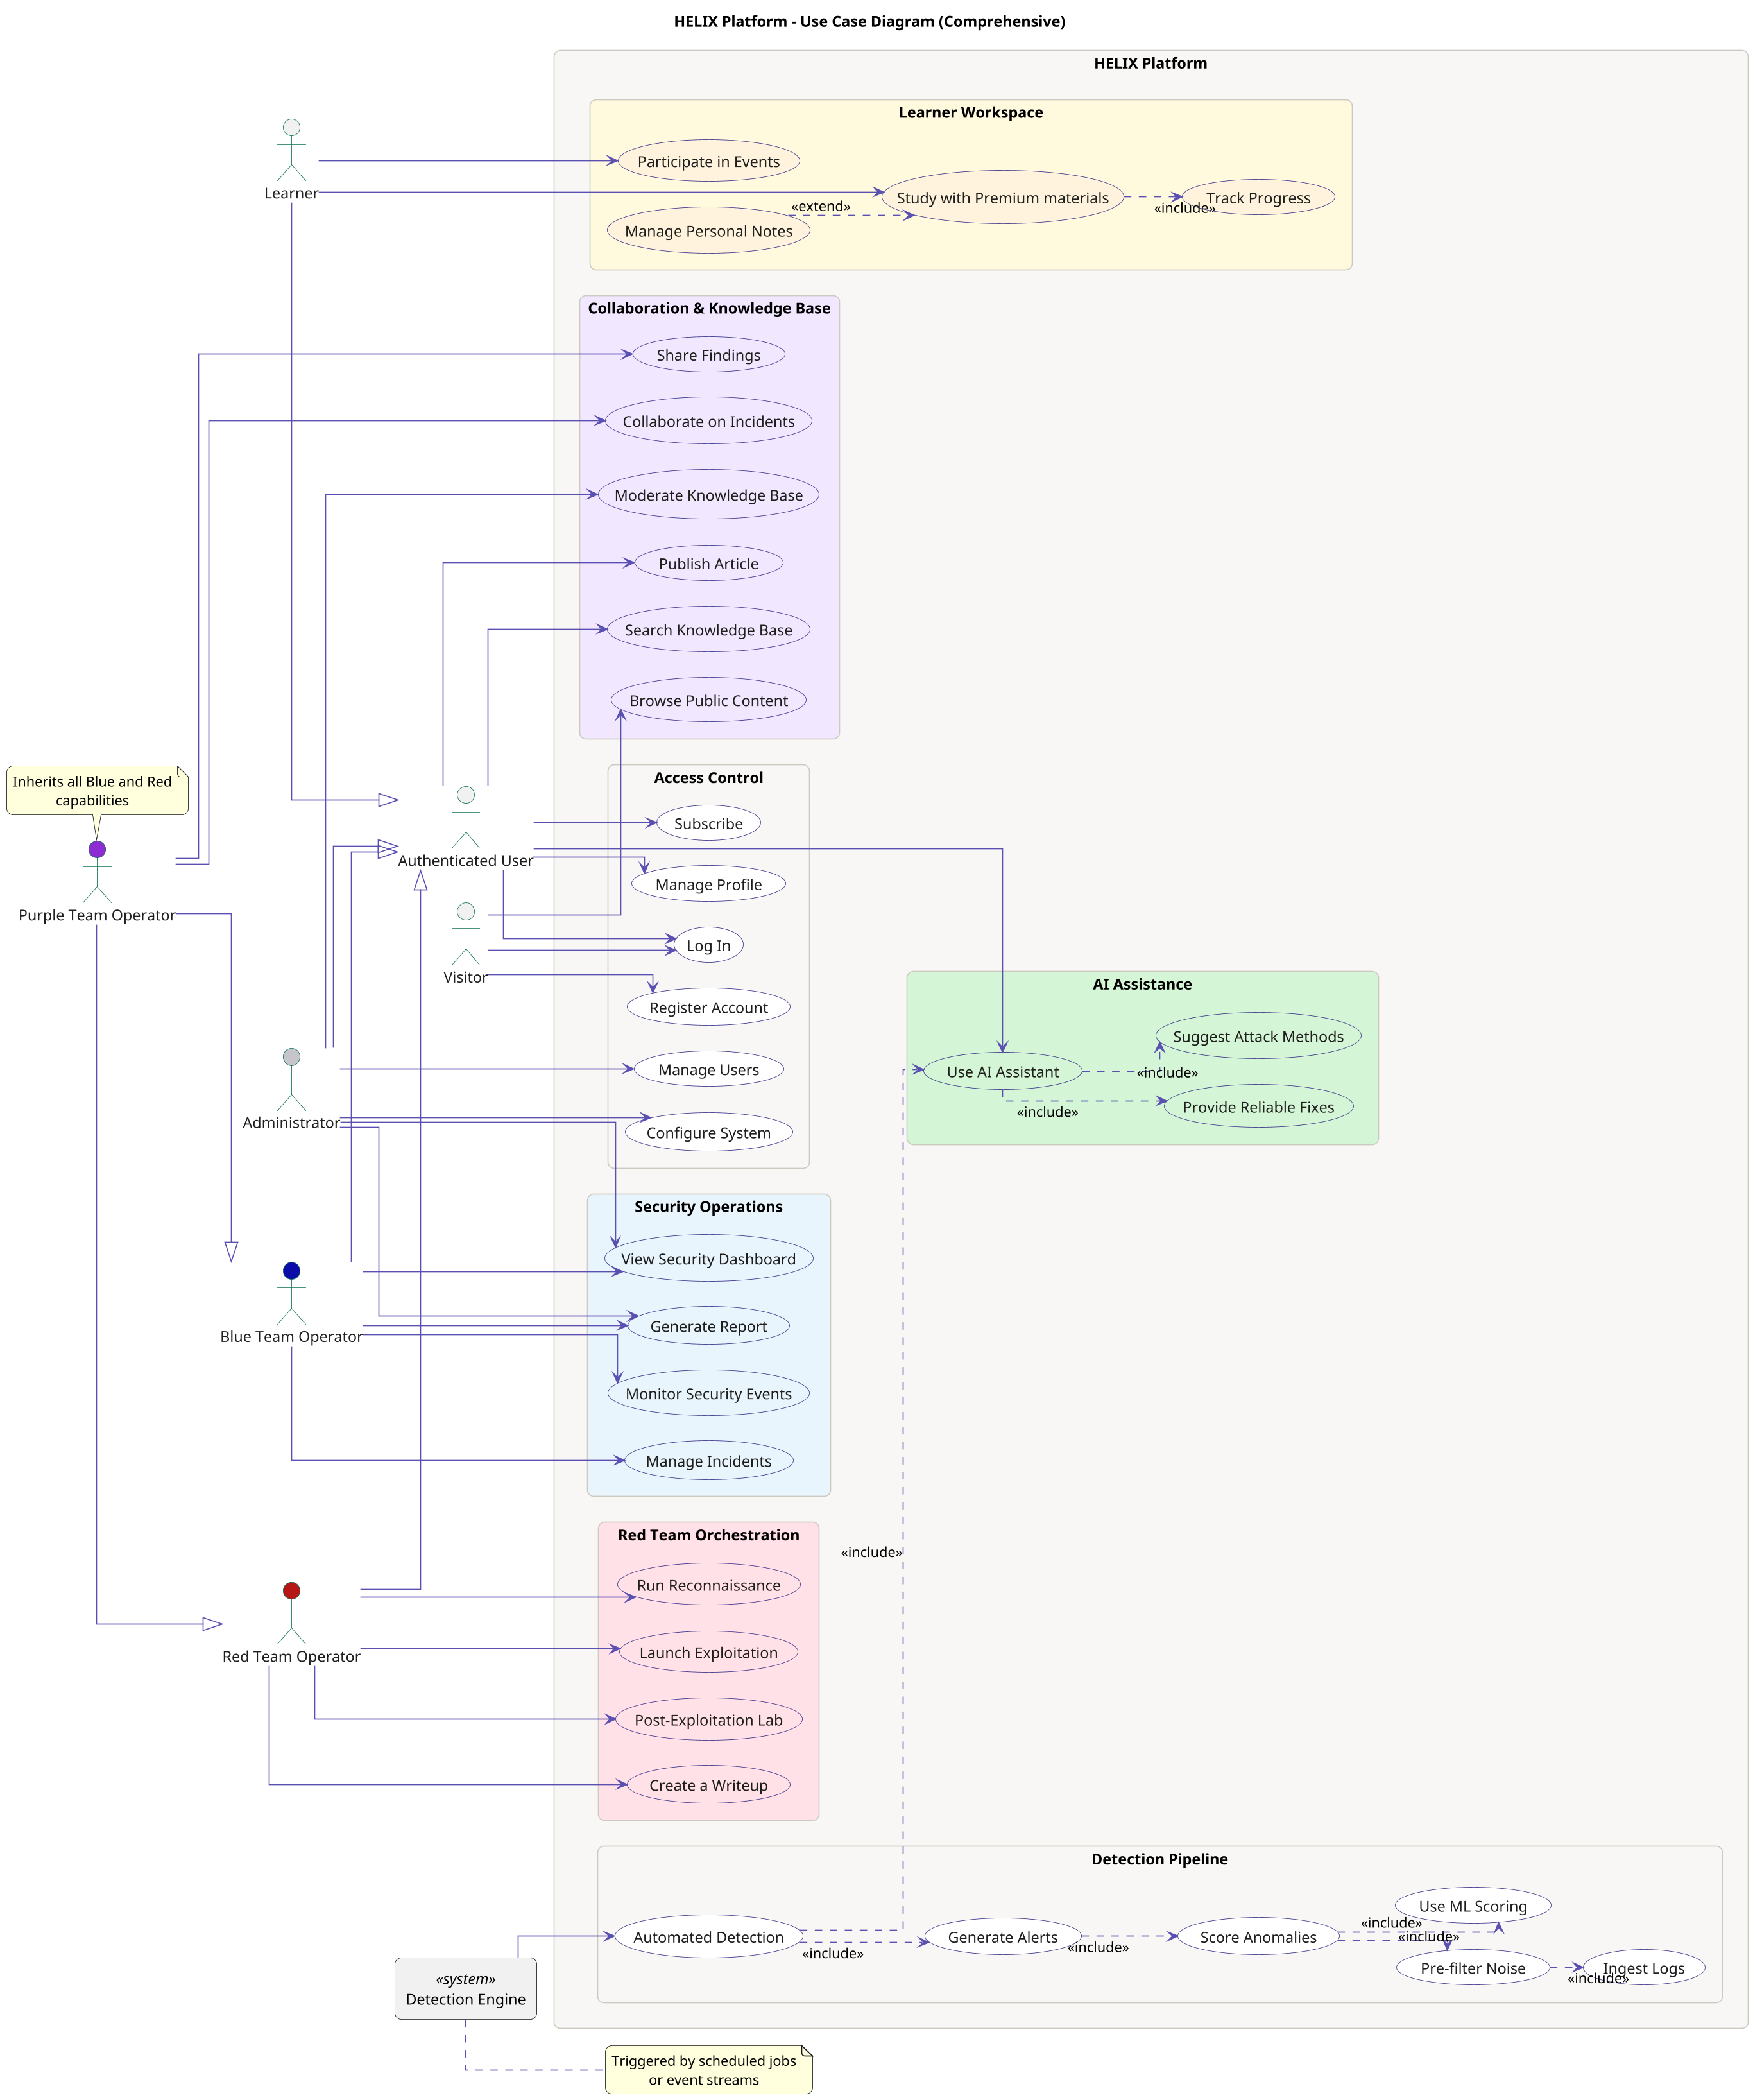
\includegraphics[width=\textwidth]{usecase_detailed.png}
    \caption{HELIX Platform – Use Case Diagram (Comprehensive)}
    \label{fig:usecase_detailed}
\end{figure}

\vspace{0.5cm}
\noindent
\textit{\textbf{Figure Notes:} Actor generalisation arrows show inheritance (e.g., Purple Team Operator inherits from both Blue Team Operator and Red Team Operator). Use case relationships use \texttt{<<include>>} and \texttt{<<extend>>} stereotypes. The Detection Engine is a system actor outside the system boundary.}
\clearpage

% ══════════════════════════════════════════════════════════════════════════
% CHAPTER 1 – ACCESS CONTROL
% ══════════════════════════════════════════════════════════════════════════
\chapter{Access Control}

\section{UC-01 -- Register Account}
\begin{ucbox}{UC-01 \quad Register Account}
    \ucfield{Actors}{Visitor (primary)}
    \ucfield{Preconditions}{User has no existing HELIX account.}
    \ucfield{Postconditions}{A new Learner account is created; user can log in.}
    \textbf{\color{helixpurplemid}Main Scenario:}
    \begin{enumerate}
        \item Visitor opens the registration form.
        \item Visitor submits username, email, and password.
        \item System validates input (unique username, password strength).
        \item System hashes the password (bcrypt) and persists the account.
        \item System confirms registration success.
    \end{enumerate}
    \textbf{\color{helixpurplemid}Alternatives:}
    \begin{itemize}
        \item \textbf{[Alt-A]} Username already exists $\rightarrow$ error displayed.
        \item \textbf{[Alt-B]} Password too weak $\rightarrow$ inline validation message.
    \end{itemize}
\end{ucbox}

\section{UC-02 -- Log In}
\begin{ucbox}{UC-02 \quad Log In}
    \ucfield{Actors}{Visitor (initiates); Authenticated User (inherits)}
    \ucfield{Preconditions}{User has a registered, active account.}
    \ucfield{Postconditions}{A valid session is created; user redirected to role dashboard.}
    \textbf{\color{helixpurplemid}Main Scenario:}
    \begin{enumerate}
        \item User submits username and password.
        \item System validates credentials against stored bcrypt hash.
        \item System creates a PHP session with role information.
        \item User is redirected to the role-appropriate dashboard.
    \end{enumerate}
    \textbf{\color{helixpurplemid}Alternatives:}
    \begin{itemize}
        \item \textbf{[Alt-A]} Invalid credentials $\rightarrow$ error message displayed.
        \item \textbf{[Alt-B]} Account deactivated $\rightarrow$ access denied.
    \end{itemize}
\end{ucbox}

\section{UC-03 -- Manage Profile}
\begin{ucbox}{UC-03 \quad Manage Profile}
    \ucfield{Actors}{Authenticated User (all concrete roles inherit)}
    \ucfield{Preconditions}{User is logged in with a valid session.}
    \ucfield{Postconditions}{Profile information updated and persisted.}
    \textbf{\color{helixpurplemid}Main Scenario:}
    \begin{enumerate}
        \item User navigates to profile settings.
        \item User modifies fields (display name, email, password).
        \item System validates and applies changes.
    \end{enumerate}
    \textbf{\color{helixpurplemid}Alternatives:}
    \begin{itemize}
        \item \textbf{[Alt-A]} New email already in use $\rightarrow$ validation error.
        \item \textbf{[Alt-B]} Password mismatch $\rightarrow$ update blocked.
    \end{itemize}
\end{ucbox}

\section{UC-04 -- Manage Users}
\begin{ucbox}{UC-04 \quad Manage Users}
    \ucfield{Actors}{Administrator (primary)}
    \ucfield{Preconditions}{Admin is authenticated.}
    \ucfield{Postconditions}{User account created, deactivated, or role-reassigned.}
    \textbf{\color{helixpurplemid}Main Scenario:}
    \begin{enumerate}
        \item Admin opens the user management panel.
        \item Admin selects an action: create, edit role, or deactivate.
        \item System applies the change and logs it to the audit trail.
    \end{enumerate}
    \textbf{\color{helixpurplemid}Alternatives:}
    \begin{itemize}
        \item \textbf{[Alt-A]} Admin tries to deactivate themselves $\rightarrow$ rejected.
        \item \textbf{[Alt-B]} Target user is logged in $\rightarrow$ session invalidated.
    \end{itemize}
\end{ucbox}

\section{UC-05 -- Configure System}
\begin{ucbox}{UC-05 \quad Configure System}
    \ucfield{Actors}{Administrator (primary)}
    \ucfield{Preconditions}{Admin is authenticated.}
    \ucfield{Postconditions}{System parameters (detection thresholds, API keys, retention) updated.}
    \textbf{\color{helixpurplemid}Main Scenario:}
    \begin{enumerate}
        \item Admin navigates to system configuration.
        \item Admin modifies parameters.
        \item System validates and saves; affected services reload.
    \end{enumerate}
    \textbf{\color{helixpurplemid}Alternatives:}
    \begin{itemize}
        \item \textbf{[Alt-A]} Invalid value $\rightarrow$ validation error.
        \item \textbf{[Alt-B]} API key incorrect $\rightarrow$ flagged on next use.
    \end{itemize}
\end{ucbox}

\section{UC-06 -- Subscribe}
\begin{ucbox}{UC-06 \quad Subscribe}
    \ucfield{Actors}{Authenticated User (primary)}
    \ucfield{Preconditions}{User is logged in. A subscription plan is available.}
    \ucfield{Postconditions}{User subscription tier upgraded; premium features unlocked.}
    \textbf{\color{helixpurplemid}Main Scenario:}
    \begin{enumerate}
        \item User navigates to the subscription page.
        \item User selects a plan and confirms.
        \item System records the subscription and updates feature access.
    \end{enumerate}
    \textbf{\color{helixpurplemid}Alternatives:}
    \begin{itemize}
        \item \textbf{[Alt-A]} Already subscribed $\rightarrow$ current plan shown.
    \end{itemize}
\end{ucbox}

% ══════════════════════════════════════════════════════════════════════════
% CHAPTER 2 – SECURITY OPERATIONS
% ══════════════════════════════════════════════════════════════════════════
\chapter{Security Operations}

\section{UC-07 -- View Security Dashboard}
\begin{ucbox}{UC-07 \quad View Security Dashboard}
    \ucfield{Actors}{Administrator, Blue Team Operator, Red Team Operator, Purple Team Operator, Learner}
    \ucfield{Preconditions}{User is authenticated. At least one security event exists.}
    \ucfield{Postconditions}{Dashboard displayed with live metrics; no state modified.}
    \textbf{\color{helixpurplemid}Main Scenario:}
    \begin{enumerate}
        \item User navigates to the Security Dashboard.
        \item System fetches metrics: active alerts by severity, 24-hour timeline, open incidents.
        \item Dashboard renders role-appropriate content.
    \end{enumerate}
    \textbf{\color{helixpurplemid}Alternatives:}
    \begin{itemize}
        \item \textbf{[Alt-A]} No events exist $\rightarrow$ empty state with guidance displayed.
        \item \textbf{[Alt-B]} Learner view $\rightarrow$ learning-oriented metrics shown.
    \end{itemize}
\end{ucbox}

\section{UC-08 -- Monitor Security Events}
\begin{ucbox}{UC-08 \quad Monitor Security Events}
    \ucfield{Actors}{Blue Team Operator (primary), Purple Team Operator}
    \ucfield{Preconditions}{User is authenticated. Log events are available.}
    \ucfield{Postconditions}{Filtered list of security events displayed.}
    \textbf{\color{helixpurplemid}Main Scenario:}
    \begin{enumerate}
        \item Operator opens the event monitoring view.
        \item Operator applies filters: severity, date range, source IP, event type.
        \item System returns matching events with enrichment data.
        \item Operator reviews details and may escalate to an incident.
    \end{enumerate}
    \textbf{\color{helixpurplemid}Alternatives:}
    \begin{itemize}
        \item \textbf{[Alt-A]} No events match $\rightarrow$ empty result; operator adjusts criteria.
    \end{itemize}
\end{ucbox}

\section{UC-09 -- Manage Incidents}
\begin{ucbox}{UC-09 \quad Manage Incidents}
    \ucfield{Actors}{Blue Team Operator (primary), Purple Team Operator, Administrator}
    \ucfield{Preconditions}{User is authenticated. At least one alert exists.}
    \ucfield{Postconditions}{Incident created or updated; status transition logged.}
    \textbf{\color{helixpurplemid}Main Scenario:}
    \begin{enumerate}
        \item Operator selects alerts and creates an incident.
        \item System assigns status \texttt{Open} with creation timestamp.
        \item Operator transitions status: Open $\rightarrow$ Investigating $\rightarrow$ Resolved, adding notes.
        \item Each change recorded in the incident timeline.
    \end{enumerate}
    \textbf{\color{helixpurplemid}Alternatives:}
    \begin{itemize}
        \item \textbf{[Alt-A]} Invalid transition $\rightarrow$ rejected; allowed transitions shown.
    \end{itemize}
\end{ucbox}

\section{UC-10 -- Generate Report}
\begin{ucbox}{UC-10 \quad Generate Report}
    \ucfield{Actors}{Blue Team Operator (primary), Administrator}
    \ucfield{Preconditions}{User is authenticated. At least one incident or alert exists.}
    \ucfield{Postconditions}{Structured PDF report generated and available for download.}
    \textbf{\color{helixpurplemid}Main Scenario:}
    \begin{enumerate}
        \item User selects scope: single incident, date range, or summary.
        \item System compiles data: timeline, severity distribution, recommendations.
        \item System generates a PDF and provides a download link.
    \end{enumerate}
    \textbf{\color{helixpurplemid}Alternatives:}
    \begin{itemize}
        \item \textbf{[Alt-A]} No data in scope $\rightarrow$ warning; prompt to adjust scope.
    \end{itemize}
\end{ucbox}

% ══════════════════════════════════════════════════════════════════════════
% CHAPTER 3 – DETECTION PIPELINE
% ══════════════════════════════════════════════════════════════════════════
\chapter{Detection Pipeline}

The Detection Engine pipeline is a chain of \texttt{<<include>>} relationships:
UC-11 (Automated Detection) includes UC-15 (Generate Alerts) $\rightarrow$ UC-14 (Score Anomalies) $\rightarrow$ UC-13 (Pre-filter Noise) $\rightarrow$ UC-12 (Ingest Logs).
UC-14 also includes UC-16 (Use ML Scoring). UC-11 includes UC-31 (Use AI Assistant).

\section{UC-11 -- Automated Detection}
\begin{ucbox}{UC-11 \quad Automated Detection}
    \ucfield{Actors}{Detection Engine (primary system actor)}
    \ucfield{Preconditions}{Detection Engine is running. Log sources are reachable.}
    \ucfield{Postconditions}{Alerts generated for anomalous events; pipeline completed.}
    \textbf{\color{helixpurplemid}Main Scenario:}
    \begin{enumerate}
        \item Detection Engine triggered by scheduler or event stream.
        \item \texttt{<<include>>} UC-12 -- Ingest Logs.
        \item \texttt{<<include>>} UC-13 -- Pre-filter Noise.
        \item \texttt{<<include>>} UC-14 -- Score Anomalies (includes UC-16).
        \item \texttt{<<include>>} UC-15 -- Generate Alerts for HIGH/CRITICAL.
        \item \texttt{<<include>>} UC-31 -- Use AI Assistant for enrichment.
        \item System notifies assigned analysts.
    \end{enumerate}
    \textbf{\color{helixpurplemid}Alternatives:}
    \begin{itemize}
        \item \textbf{[Alt-A]} Log source unreachable $\rightarrow$ error logged; pipeline continues.
        \item \textbf{[Alt-B]} ML model unavailable $\rightarrow$ rule-based detection continues.
        \item \textbf{[Alt-C]} AI service offline $\rightarrow$ alerts generated without AI enrichment.
    \end{itemize}
\end{ucbox}

\section{UC-12 -- Ingest Logs}
\begin{ucbox}{UC-12 \quad Ingest Logs \textnormal{(included by UC-13)}}
    \ucfield{Actors}{Detection Engine}
    \ucfield{Preconditions}{Log source accessible; parser registered.}
    \ucfield{Postconditions}{Raw logs parsed and normalised as structured entries.}
    \textbf{\color{helixpurplemid}Main Scenario:}
    \begin{enumerate}
        \item Engine reads raw logs (Syslog, JSON, Apache, Windows Event Log).
        \item Parser selects appropriate format handler.
        \item Each entry normalised into structured fields and written to staging store.
    \end{enumerate}
    \textbf{\color{helixpurplemid}Alternatives:}
    \begin{itemize}
        \item \textbf{[Alt-A]} Unknown format $\rightarrow$ tagged as unparseable; flagged for review.
    \end{itemize}
\end{ucbox}

\section{UC-13 -- Pre-filter Noise}
\begin{ucbox}{UC-13 \quad Pre-filter Noise \textnormal{(included by UC-14)}}
    \ucfield{Actors}{Detection Engine}
    \ucfield{Preconditions}{Normalised log entries in staging store.}
    \ucfield{Postconditions}{Low-signal events suppressed; high-signal events forwarded.}
    \textbf{\color{helixpurplemid}Main Scenario:}
    \begin{enumerate}
        \item Noise filter evaluates each log entry.
        \item Duplicate or benign patterns discarded; suppression reason logged.
        \item Remaining events forwarded to scoring stage.
    \end{enumerate}
    \textbf{\color{helixpurplemid}Alternatives:}
    \begin{itemize}
        \item \textbf{[Alt-A]} Filter unavailable $\rightarrow$ all events pass through.
    \end{itemize}
\end{ucbox}

\section{UC-14 -- Score Anomalies}
\begin{ucbox}{UC-14 \quad Score Anomalies \textnormal{(included by UC-15)}}
    \ucfield{Actors}{Detection Engine}
    \ucfield{Preconditions}{Filtered events available. ML model loaded.}
    \ucfield{Postconditions}{Each event receives severity: LOW, MEDIUM, HIGH, or CRITICAL.}
    \textbf{\color{helixpurplemid}Main Scenario:}
    \begin{enumerate}
        \item \texttt{<<include>>} UC-16 -- Use ML Scoring (Isolation Forest).
        \item Anomaly score mapped to severity per thresholds.
        \item Scored events written to detection store.
    \end{enumerate}
    \textbf{\color{helixpurplemid}Alternatives:}
    \begin{itemize}
        \item \textbf{[Alt-A]} ML model fails $\rightarrow$ rule-based fallback assigns severity.
    \end{itemize}
\end{ucbox}

\section{UC-15 -- Generate Alerts}
\begin{ucbox}{UC-15 \quad Generate Alerts \textnormal{(included by UC-11)}}
    \ucfield{Actors}{Detection Engine}
    \ucfield{Preconditions}{UC-14 completed; HIGH or CRITICAL events exist.}
    \ucfield{Postconditions}{Alert records created; analysts notified; audit log written.}
    \textbf{\color{helixpurplemid}Main Scenario:}
    \begin{enumerate}
        \item System selects events scored HIGH or CRITICAL.
        \item For each, an alert record created with timestamp, source IP, severity.
        \item System enriches alert with GeoIP and reputation data.
        \item Notifications dispatched to Blue Team Operators.
    \end{enumerate}
    \textbf{\color{helixpurplemid}Alternatives:}
    \begin{itemize}
        \item \textbf{[Alt-A]} Enrichment APIs unreachable $\rightarrow$ alert created without enrichment.
    \end{itemize}
\end{ucbox}

\section{UC-16 -- Use ML Scoring}
\begin{ucbox}{UC-16 \quad Use ML Scoring \textnormal{(included by UC-14)}}
    \ucfield{Actors}{Detection Engine}
    \ucfield{Preconditions}{Isolation Forest model loaded and up to date.}
    \ucfield{Postconditions}{Each event receives a continuous anomaly score.}
    \textbf{\color{helixpurplemid}Main Scenario:}
    \begin{enumerate}
        \item Engine constructs feature vector per event (event frequency, error rate, time-of-day, source IP diversity).
        \item Isolation Forest returns anomaly score.
        \item Score forwarded to UC-14 for severity mapping.
    \end{enumerate}
    \textbf{\color{helixpurplemid}Alternatives:}
    \begin{itemize}
        \item \textbf{[Alt-A]} Feature extraction fails $\rightarrow$ event scored MEDIUM by default.
    \end{itemize}
\end{ucbox}

% ══════════════════════════════════════════════════════════════════════════
% CHAPTER 4 – RED TEAM ORCHESTRATION
% ══════════════════════════════════════════════════════════════════════════
\chapter{Red Team Orchestration}

\section{UC-17 -- Run Reconnaissance}
\begin{ucbox}{UC-17 \quad Run Reconnaissance}
    \ucfield{Actors}{Red Team Operator (primary), Purple Team Operator}
    \ucfield{Preconditions}{User authenticated with Red Team role. Legal consent accepted. Target in scope.}
    \ucfield{Postconditions}{Reconnaissance results persisted and viewable.}
    \textbf{\color{helixpurplemid}Main Scenario:}
    \begin{enumerate}
        \item Operator selects tool (nmap, WHOIS, OSINT).
        \item Operator specifies target and scan parameters.
        \item System executes tool server-side; results streamed back.
        \item Results normalised and stored in scan history.
    \end{enumerate}
    \textbf{\color{helixpurplemid}Alternatives:}
    \begin{itemize}
        \item \textbf{[Alt-A]} Tool timeout $\rightarrow$ partial results stored; error flagged.
        \item \textbf{[Alt-B]} Target out of scope $\rightarrow$ execution blocked; attempt logged.
    \end{itemize}
\end{ucbox}

\section{UC-18 -- Launch Exploitation}
\begin{ucbox}{UC-18 \quad Launch Exploitation}
    \ucfield{Actors}{Red Team Operator (primary), Purple Team Operator}
    \ucfield{Preconditions}{Reconnaissance complete. Legal consent accepted.}
    \ucfield{Postconditions}{Exploitation result logged (success or failure).}
    \textbf{\color{helixpurplemid}Main Scenario:}
    \begin{enumerate}
        \item Operator selects a vulnerability from recon findings.
        \item Operator configures an exploit module.
        \item System executes exploit and captures result.
        \item Result (success/failure, CVE reference) persisted.
    \end{enumerate}
    \textbf{\color{helixpurplemid}Alternatives:}
    \begin{itemize}
        \item \textbf{[Alt-A]} Exploit fails $\rightarrow$ failure logged; alternative suggested.
        \item \textbf{[Alt-B]} Consent not accepted $\rightarrow$ features blocked.
    \end{itemize}
\end{ucbox}

\section{UC-19 -- Post-Exploitation Lab}
\begin{ucbox}{UC-19 \quad Post-Exploitation Lab}
    \ucfield{Actors}{Red Team Operator (primary), Purple Team Operator}
    \ucfield{Preconditions}{Successful exploitation or lab environment available.}
    \ucfield{Postconditions}{Post-exploitation actions logged for analysis.}
    \textbf{\color{helixpurplemid}Main Scenario:}
    \begin{enumerate}
        \item Operator enters the post-exploitation lab environment.
        \item Operator performs actions: privilege escalation, lateral movement, exfiltration simulation.
        \item Each action recorded for blue team awareness.
    \end{enumerate}
    \textbf{\color{helixpurplemid}Alternatives:}
    \begin{itemize}
        \item \textbf{[Alt-A]} Lab environment unavailable $\rightarrow$ retry after environment reset.
    \end{itemize}
\end{ucbox}

\section{UC-20 -- Create a Writeup}
\begin{ucbox}{UC-20 \quad Create a Writeup}
    \ucfield{Actors}{Red Team Operator (primary), Purple Team Operator}
    \ucfield{Preconditions}{User authenticated. An operation or CTF result exists.}
    \ucfield{Postconditions}{Writeup submitted for moderation; visible upon approval.}
    \textbf{\color{helixpurplemid}Main Scenario:}
    \begin{enumerate}
        \item Operator opens the writeup editor.
        \item Operator drafts content, attaches screenshots and scan results.
        \item Operator submits; system tags and queues for Admin moderation.
    \end{enumerate}
    \textbf{\color{helixpurplemid}Alternatives:}
    \begin{itemize}
        \item \textbf{[Alt-A]} Writeup rejected $\rightarrow$ operator notified with reason; can revise.
    \end{itemize}
\end{ucbox}

% ══════════════════════════════════════════════════════════════════════════
% CHAPTER 5 – COLLABORATION & KNOWLEDGE BASE
% ══════════════════════════════════════════════════════════════════════════
\chapter{Collaboration \& Knowledge Base}

\section{UC-21 -- Browse Public Content}
\begin{ucbox}{UC-21 \quad Browse Public Content}
    \ucfield{Actors}{Visitor (primary)}
    \ucfield{Preconditions}{None. User is unauthenticated.}
    \ucfield{Postconditions}{Public content displayed; no session created.}
    \textbf{\color{helixpurplemid}Main Scenario:}
    \begin{enumerate}
        \item Visitor navigates to the HELIX public homepage.
        \item System renders publicly available articles, writeups, and platform features.
        \item Visitor browses content without logging in.
    \end{enumerate}
    \textbf{\color{helixpurplemid}Alternatives:}
    \begin{itemize}
        \item \textbf{[Alt-A]} Visitor accesses restricted page $\rightarrow$ redirected to login.
    \end{itemize}
\end{ucbox}

\section{UC-22 -- Search Knowledge Base}
\begin{ucbox}{UC-22 \quad Search Knowledge Base}
    \ucfield{Actors}{Authenticated User (all concrete roles inherit)}
    \ucfield{Preconditions}{User is logged in. Published articles exist.}
    \ucfield{Postconditions}{Matching articles displayed; no state changed.}
    \textbf{\color{helixpurplemid}Main Scenario:}
    \begin{enumerate}
        \item User enters a search query (keyword, tag, or difficulty).
        \item System performs full-text search and returns ranked results.
        \item User selects and reads an article.
    \end{enumerate}
    \textbf{\color{helixpurplemid}Alternatives:}
    \begin{itemize}
        \item \textbf{[Alt-A]} No results $\rightarrow$ system suggests related tags.
    \end{itemize}
\end{ucbox}

\section{UC-23 -- Publish Article}
\begin{ucbox}{UC-23 \quad Publish Article}
    \ucfield{Actors}{Authenticated User (all concrete roles inherit)}
    \ucfield{Preconditions}{User is logged in.}
    \ucfield{Postconditions}{Article submitted; visible after Admin moderation.}
    \textbf{\color{helixpurplemid}Main Scenario:}
    \begin{enumerate}
        \item User opens the article editor.
        \item User writes content, adds tags (topic, team, difficulty).
        \item User submits; article enters \texttt{Pending} status, queued for moderation.
        \item On approval, article becomes searchable (UC-22).
    \end{enumerate}
    \textbf{\color{helixpurplemid}Alternatives:}
    \begin{itemize}
        \item \textbf{[Alt-A]} Article flagged $\rightarrow$ user notified; draft preserved.
    \end{itemize}
\end{ucbox}

\section{UC-24 -- Collaborate on Incidents}
\begin{ucbox}{UC-24 \quad Collaborate on Incidents}
    \ucfield{Actors}{Purple Team Operator (primary)}
    \ucfield{Preconditions}{User authenticated as Purple Team. Active incident exists.}
    \ucfield{Postconditions}{Incident updated with cross-team annotations; timeline entry created.}
    \textbf{\color{helixpurplemid}Main Scenario:}
    \begin{enumerate}
        \item Operator opens an active incident.
        \item Operator adds cross-team annotations: correlating Red findings with Blue alerts.
        \item System records annotation with author and timestamp.
    \end{enumerate}
    \textbf{\color{helixpurplemid}Alternatives:}
    \begin{itemize}
        \item \textbf{[Alt-A]} Incident closed $\rightarrow$ view-only; can reopen with justification.
    \end{itemize}
\end{ucbox}

\section{UC-25 -- Share Findings}
\begin{ucbox}{UC-25 \quad Share Findings}
    \ucfield{Actors}{Purple Team Operator (primary)}
    \ucfield{Preconditions}{User authenticated as Purple Team. Completed operation or incident exists.}
    \ucfield{Postconditions}{Findings shared; notification sent.}
    \textbf{\color{helixpurplemid}Main Scenario:}
    \begin{enumerate}
        \item Operator selects findings (scan results, timeline, writeup) to share.
        \item Operator designates recipients (team or individual).
        \item System packages findings and notifies recipients in-app.
    \end{enumerate}
    \textbf{\color{helixpurplemid}Alternatives:}
    \begin{itemize}
        \item \textbf{[Alt-A]} Recipient has insufficient clearance $\rightarrow$ sharing blocked.
    \end{itemize}
\end{ucbox}

\section{UC-26 -- Moderate Knowledge Base}
\begin{ucbox}{UC-26 \quad Moderate Knowledge Base}
    \ucfield{Actors}{Administrator (primary)}
    \ucfield{Preconditions}{Admin authenticated. Articles pending review exist.}
    \ucfield{Postconditions}{Article approved (published), rejected, or archived.}
    \textbf{\color{helixpurplemid}Main Scenario:}
    \begin{enumerate}
        \item Admin opens the moderation queue.
        \item Admin reviews each pending article for guideline compliance.
        \item Admin approves $\rightarrow$ article goes live; or rejects with reason $\rightarrow$ author notified.
    \end{enumerate}
    \textbf{\color{helixpurplemid}Alternatives:}
    \begin{itemize}
        \item \textbf{[Alt-A]} Admin archives published article $\rightarrow$ removed from search, preserved.
        \item \textbf{[Alt-B]} Admin deletes article $\rightarrow$ requires confirmation.
    \end{itemize}
\end{ucbox}

% ══════════════════════════════════════════════════════════════════════════
% CHAPTER 6 – LEARNER WORKSPACE
% ══════════════════════════════════════════════════════════════════════════
\chapter{Learner Workspace}

\section{UC-27 -- Study with Premium Materials}
\begin{ucbox}{UC-27 \quad Study with Premium Materials}
    \ucfield{Actors}{Learner (primary)}
    \ucfield{Preconditions}{Learner authenticated with active subscription. Premium content exists.}
    \ucfield{Postconditions}{Premium module accessed; progress updated (UC-29 included).}
    \textbf{\color{helixpurplemid}Main Scenario:}
    \begin{enumerate}
        \item Learner navigates to the premium learning section.
        \item Learner selects a module (video, lab, quiz).
        \item System renders content and records access.
        \item \texttt{<<include>>} UC-29 -- Track Progress: completion updated.
    \end{enumerate}
    \textbf{\color{helixpurplemid}Alternatives:}
    \begin{itemize}
        \item \textbf{[Alt-A]} Subscription expired $\rightarrow$ access blocked; redirect to subscribe.
        \item \textbf{[Alt-B]} Learner wants notes $\rightarrow$ \texttt{<<extend>>} UC-28.
    \end{itemize}
\end{ucbox}

\section{UC-28 -- Manage Personal Notes}
\begin{ucbox}{UC-28 \quad Manage Personal Notes \textnormal{(\texttt{<<extend>>} UC-27)}}
    \ucfield{Actors}{Learner (primary)}
    \ucfield{Preconditions}{Learner authenticated. A module or article is open.}
    \ucfield{Postconditions}{Note created, updated, or deleted; data strictly private.}
    \textbf{\color{helixpurplemid}Main Scenario:}
    \begin{enumerate}
        \item Learner opens the Notes panel alongside a module or article.
        \item Learner creates, edits, or deletes a note.
        \item System persists the note, linked to the content; visible only to owner and Admin.
    \end{enumerate}
    \textbf{\color{helixpurplemid}Alternatives:}
    \begin{itemize}
        \item \textbf{[Alt-A]} Learner searches notes by keyword $\rightarrow$ matching notes displayed.
    \end{itemize}
\end{ucbox}

\section{UC-29 -- Track Progress}
\begin{ucbox}{UC-29 \quad Track Progress \textnormal{(included by UC-27)}}
    \ucfield{Actors}{Learner (indirect, via UC-27)}
    \ucfield{Preconditions}{Learner completes or accesses a module/exercise.}
    \ucfield{Postconditions}{Progress log updated; dashboard refreshed.}
    \textbf{\color{helixpurplemid}Main Scenario:}
    \begin{enumerate}
        \item System records completed module, quiz score, or CTF flag in progress log.
        \item Learner's dashboard updated with new completion percentage.
    \end{enumerate}
    \textbf{\color{helixpurplemid}Alternatives:}
    \begin{itemize}
        \item \textbf{[Alt-A]} Module already completed $\rightarrow$ marked as revisited; no duplicate entry.
    \end{itemize}
\end{ucbox}

\section{UC-30 -- Participate in Events}
\begin{ucbox}{UC-30 \quad Participate in Events}
    \ucfield{Actors}{Learner (primary)}
    \ucfield{Preconditions}{Learner authenticated. An active event (CTF, webinar, challenge) is live.}
    \ucfield{Postconditions}{Learner registered for or completed the event; results logged.}
    \textbf{\color{helixpurplemid}Main Scenario:}
    \begin{enumerate}
        \item Learner browses the events calendar.
        \item Learner registers for an upcoming event or joins a live event.
        \item Learner submits flags or answers; results recorded on the leaderboard.
        \item Event completion logged in the progress tracker (via UC-29).
    \end{enumerate}
    \textbf{\color{helixpurplemid}Alternatives:}
    \begin{itemize}
        \item \textbf{[Alt-A]} Event at capacity $\rightarrow$ learner added to waitlist.
        \item \textbf{[Alt-B]} Deadline passed $\rightarrow$ registration closed; archived materials viewable.
    \end{itemize}
\end{ucbox}

% ══════════════════════════════════════════════════════════════════════════
% CHAPTER 7 – AI ASSISTANCE
% ══════════════════════════════════════════════════════════════════════════
\chapter{AI Assistance}

\section{UC-31 -- Use AI Assistant}
\begin{ucbox}{UC-31 \quad Use AI Assistant}
    \ucfield{Actors}{Authenticated User (all concrete roles inherit)}
    \ucfield{Preconditions}{User is logged in. OpenAI API available. Alert or query context exists.}
    \ucfield{Postconditions}{AI-generated explanation, remediation, or attack suggestion returned.}
    \textbf{\color{helixpurplemid}Main Scenario:}
    \begin{enumerate}
        \item User opens the AI Assistant panel (from alert, incident, or freeform chat).
        \item System constructs a prompt with alert context and relevant log data.
        \item \texttt{<<include>>} UC-32 -- Provide Reliable Fixes.
        \item \texttt{<<include>>} UC-33 -- Suggest Attack Methods.
        \item AI response displayed; conversation history persisted per session.
    \end{enumerate}
    \textbf{\color{helixpurplemid}Alternatives:}
    \begin{itemize}
        \item \textbf{[Alt-A]} OpenAI API unavailable $\rightarrow$ degraded mode message displayed.
        \item \textbf{[Alt-B]} User submits CVE identifier $\rightarrow$ CVE summary returned.
    \end{itemize}
\end{ucbox}

\section{UC-32 -- Provide Reliable Fixes}
\begin{ucbox}{UC-32 \quad Provide Reliable Fixes \textnormal{(included by UC-31)}}
    \ucfield{Actors}{AI Service (internal)}
    \ucfield{Preconditions}{UC-31 initiated; alert context available.}
    \ucfield{Postconditions}{Context-specific remediation steps returned.}
    \textbf{\color{helixpurplemid}Main Scenario:}
    \begin{enumerate}
        \item OpenAI API receives alert context and queries knowledge base for matching patterns.
        \item System returns prioritised remediation checklist (patch, block IP, rotate credentials).
    \end{enumerate}
    \textbf{\color{helixpurplemid}Alternatives:}
    \begin{itemize}
        \item \textbf{[Alt-A]} No known mitigation $\rightarrow$ generic hardening guidance returned.
    \end{itemize}
\end{ucbox}

\section{UC-33 -- Suggest Attack Methods}
\begin{ucbox}{UC-33 \quad Suggest Attack Methods \textnormal{(included by UC-31)}}
    \ucfield{Actors}{AI Service (internal)}
    \ucfield{Preconditions}{UC-31 initiated; Red Team or Purple Team context detected.}
    \ucfield{Postconditions}{Relevant attack techniques returned.}
    \textbf{\color{helixpurplemid}Main Scenario:}
    \begin{enumerate}
        \item OpenAI API identifies the attack surface or target technology from context.
        \item System returns relevant attack techniques, tools, and exploitation paths.
    \end{enumerate}
    \textbf{\color{helixpurplemid}Alternatives:}
    \begin{itemize}
        \item \textbf{[Alt-A]} Legal consent not accepted $\rightarrow$ output blocked with consent prompt.
    \end{itemize}
\end{ucbox}

% ══════════════════════════════════════════════════════════════════════════
% CONCLUSION
% ══════════════════════════════════════════════════════════════════════════
\chapter*{Conclusion}
\addcontentsline{toc}{chapter}{Conclusion}

\begin{successbox}[title=Summary]
    This document provides complete textual descriptions for all \textbf{33 use cases}
    (UC-01 to UC-33) of the HELIX platform, fully aligned with the SRS and Use Case Diagram.
    All descriptions follow the academic format: \textit{Name, Actors, Preconditions,
    Postconditions, Main Scenario, and Alternative Scenarios}. The eight actors
    (Authenticated User, Administrator, Blue Team Operator, Red Team Operator,
    Purple Team Operator, Visitor, Learner, Detection Engine) are consistently applied.
\end{successbox}

\end{document}
